% !TeX encoding = UTF-8
% !TeX program = xelatex
% !TeX spellcheck = en_US

\documentclass[degree=doctor]{bnuthesis}
  % 学位 degree:
  %   doctor | master | bachelor
  % 学位类型 degree-type:
  %   academic(默认)| professional
  % 语言 language
  %   chinese(默认)
  % 字体库 fontset
  %   windows | mac | fandol | ubuntu
  % 建议终版使用 Windows 平台的字体编译


% 论文基本配置,加载宏包等全局配置
% !TeX root = ./bnuthesis-example.tex

% 论文基本信息配置

\bnusetup{
  %******************************
  % 注意:
  %   1. 配置里面不要出现空行
  %   2. 不需要的配置信息可以删除
  %   3. 建议先阅读文档中所有关于选项的说明
  %******************************
  %
  % 输出格式
  %   选择打印版(print)或用于提交的电子版(electronic),前者会插入空白页以便直接双面打印
  %
  output = electronic,
  %
  % 标题
  %   可使用“\\”命令手动控制换行
  %
  title  = {多视角信息融合的食管癌辅助诊断研究},
  title* = {Multi-Perspective Information Fusion for Esophageal Cancer Auxiliary Diagnosis Research},
  %
  % 学科门类
  %   1. 学术型
  %      - 中文
  %        需注明所属的学科门类,例如:
  %        哲学、经济学、法学、教育学、文学、历史学、理学、工学、农学、医学、
  %        军事学、管理学、艺术学
  %      - 英文
  %        博士:Doctor of Philosophy
  %        硕士:
  %          哲学、文学、历史学、法学、教育学、艺术学门类,公共管理学科
  %          填写“Master of Arts“,其它填写“Master of Science”
  %   2. 专业型
  %      直接填写专业学位的名称,例如:
  %      教育博士、工程硕士等
  %      Doctor of Education, Master of Engineering
  %   3. 本科生不需要填写
  %
  % degree-category  = {教育硕士},
  % degree-category* = {Master of Education},
  %
  % 培养单位
  %   填写所属院系的全名
  %
  department = {计算机科学与技术学院},
  %
  % 学科
  %   1. 研究生学术型学位,获得一级学科授权的学科填写一级学科名称,其他填写二级学科名称
  %   2. 本科生填写专业名称,第二学位论文需标注“(第二学位)”
  %
  discipline  = {计算机科学与技术},
  % discipline* = {Computer Science and Technology},
  %
  % 专业领域
  %   1. 设置专业领域的专业学位类别,填写相应专业领域名称
  %   2. 2019 级及之前工程硕士学位论文,在 `engineering-field` 填写相应工程领域名称
  %   3. 其他专业学位类别的学位论文无需此信息
  %
  % professional-field  = {学科教学(数学)},
  % professional-field* = {Subject Teaching(Mathematics)},
  %
  % 姓名
  %
  author  = {霍相佐},
  % author* = {Xiangzuo Huo},
  student-id = {107556521207},
  %
  % 导师
  %   中文姓名和职称之间以英文逗号“,”分开,下同
  %
  supervisor  = {田生伟, 教授},
  % supervisor* = {Professor Tian},
  % supervisor-department = {软件学院},
  %
  % 副导师
  %
  % associate-supervisor  = {陈文光, 教授},
  % associate-supervisor* = {Professor Chen Wenguang},
  %
  % 联合导师
  %
  % co-supervisor  = {某某某, 教授},
  % co-supervisor* = {Professor Mou Moumou},
  %
  % 日期
  %   使用 ISO 格式;默认为当前时间
  %
  date = {2024-03-01},
  %
  % 是否在中文封面后的空白页生成书脊(默认 false),仅博士需要。
  %
  include-spine = false,
  spine-author = {新疆大学},
  %
  % 密级和年限
  %   秘密, 机密, 绝密
  %
  % secret-level = {秘密},
  % secret-year  = {10},
  %
}

% 载入所需的宏包

% 定理类环境宏包
\usepackage{amsthm}
% 也可以使用 ntheorem
% \usepackage[amsmath,thmmarks,hyperref]{ntheorem}

\bnusetup{
  %
  % 数学字体
  % math-style = GB,  % GB | ISO | TeX
  math-font  = xits,  % stix | xits | libertinus
  % 图表编号时是否带有章节序号,默认为不带有false
  figurestables-chapternumber = false,  %false / true
}

% 可以使用 nomencl 生成符号和缩略语说明
% \usepackage{nomencl}
% \makenomenclature

% 表格加脚注
\usepackage{threeparttable}

% 表格中支持跨行
\usepackage{multirow}

% 固定宽度的表格。
% \usepackage{tabularx}

% 跨页表格
\usepackage{longtable}

% 算法
\usepackage{algorithm}
\usepackage{algorithmic}

% 量和单位
\usepackage{siunitx}

% 参考文献使用 BibTeX + natbib 宏包
% 顺序编码制
\usepackage[sort]{natbib}
\bibliographystyle{bnuthesis-numeric}

% 著者-出版年制
% \usepackage{natbib}
% \bibliographystyle{bnuthesis-author-year}

% 本科生参考文献的著录格式
% \usepackage[sort]{natbib}
% \bibliographystyle{bnuthesis-bachelor}

% 参考文献使用 BibLaTeX 宏包
% \usepackage[style=bnuthesis-numeric]{biblatex}
% \usepackage[style=bnuthesis-author-year]{biblatex}
% \usepackage[style=gb7714-2015]{biblatex}
% \usepackage[style=apa]{biblatex}
% \usepackage[style=mla-new]{biblatex}
% 声明 BibLaTeX 的数据库
% \addbibresource{ref/refs.bib}

% 定义所有的图片文件在 figures 子目录下
\graphicspath{{figures/}}

% 数学命令
\makeatletter
\newcommand\dif{%  % 微分符号
  \mathop{}\!%
  \ifbnu@math@style@TeX
    d%
  \else
    \mathrm{d}%
  \fi
}
\makeatother

% hyperref 宏包在最后调用
\usepackage{hyperref}



\begin{document}

% 封面
% \maketitle
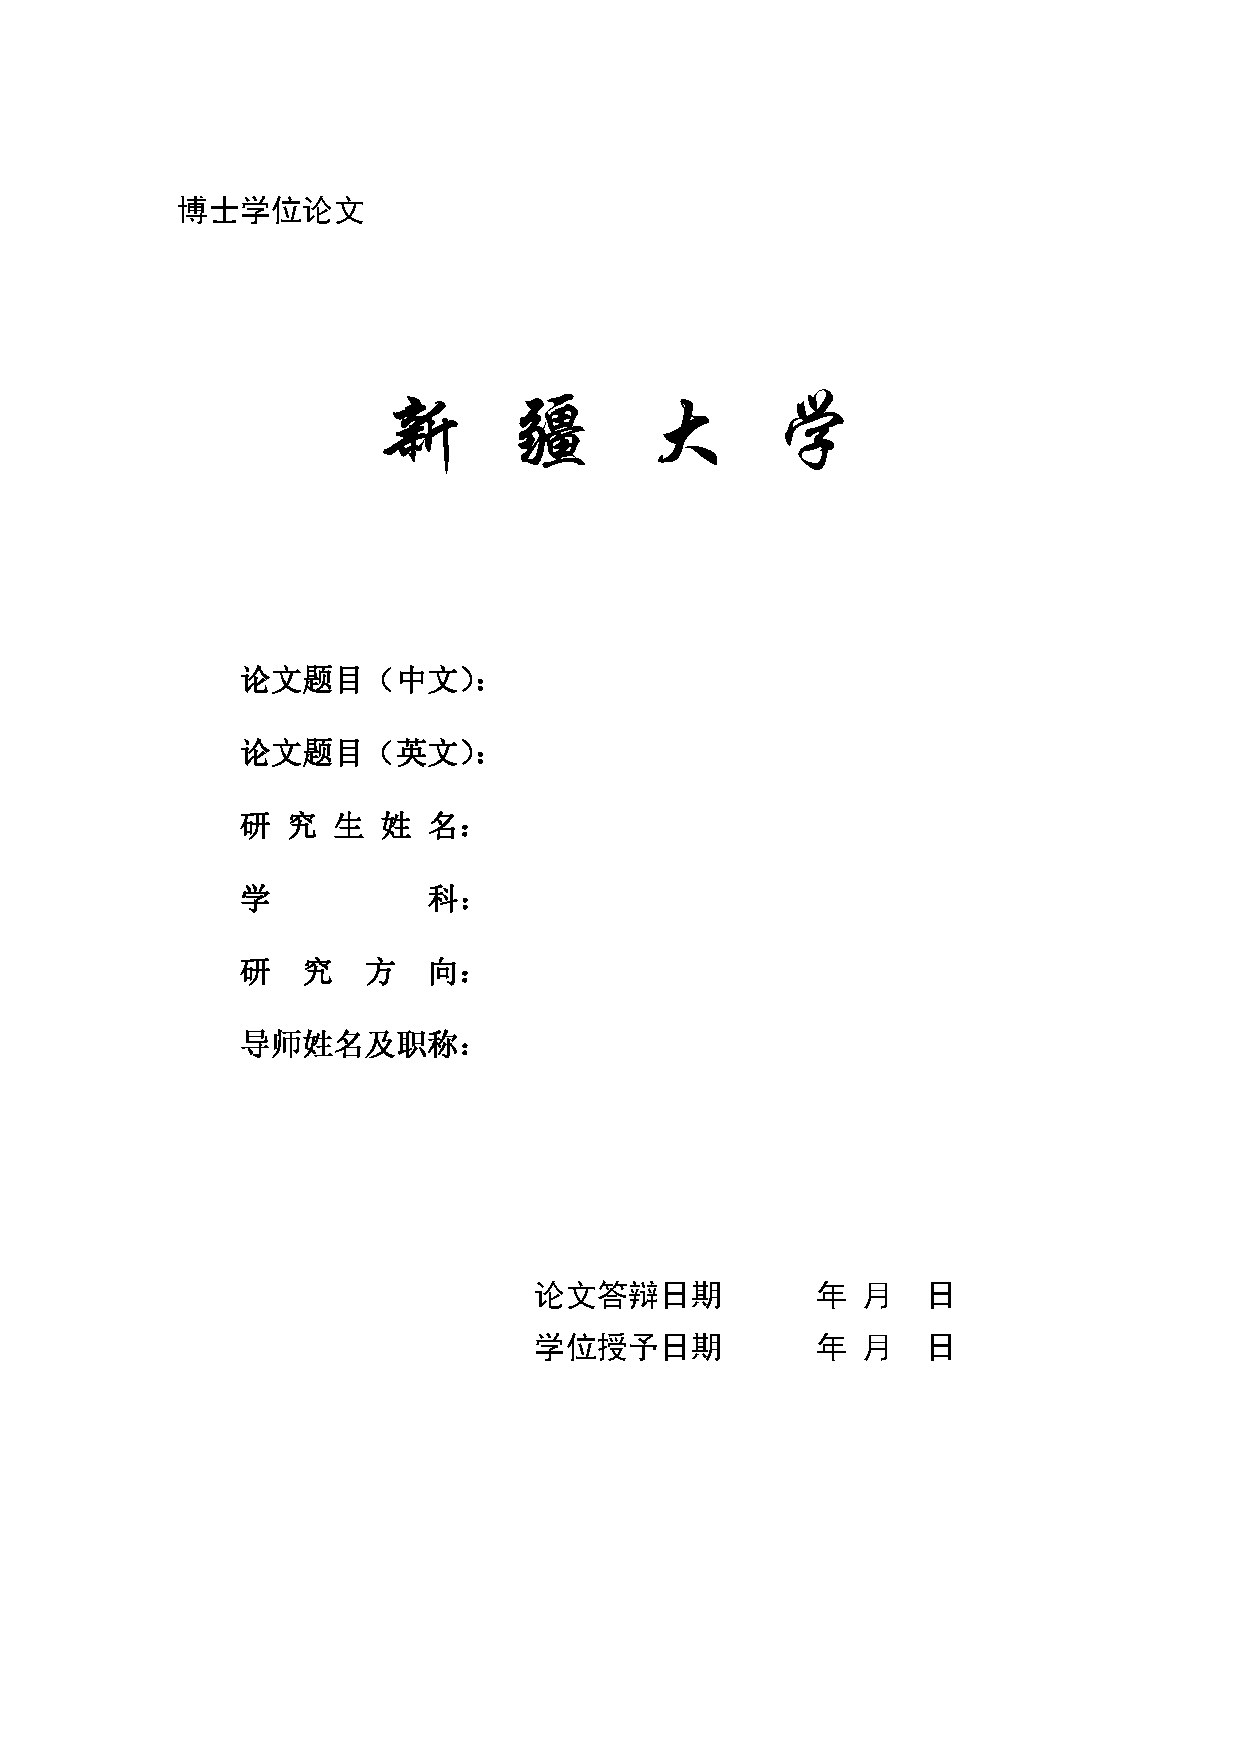
\includepdf{xju_special/xju-doc.pdf} % 博士论文封面   请填写内容后上传pdf
% 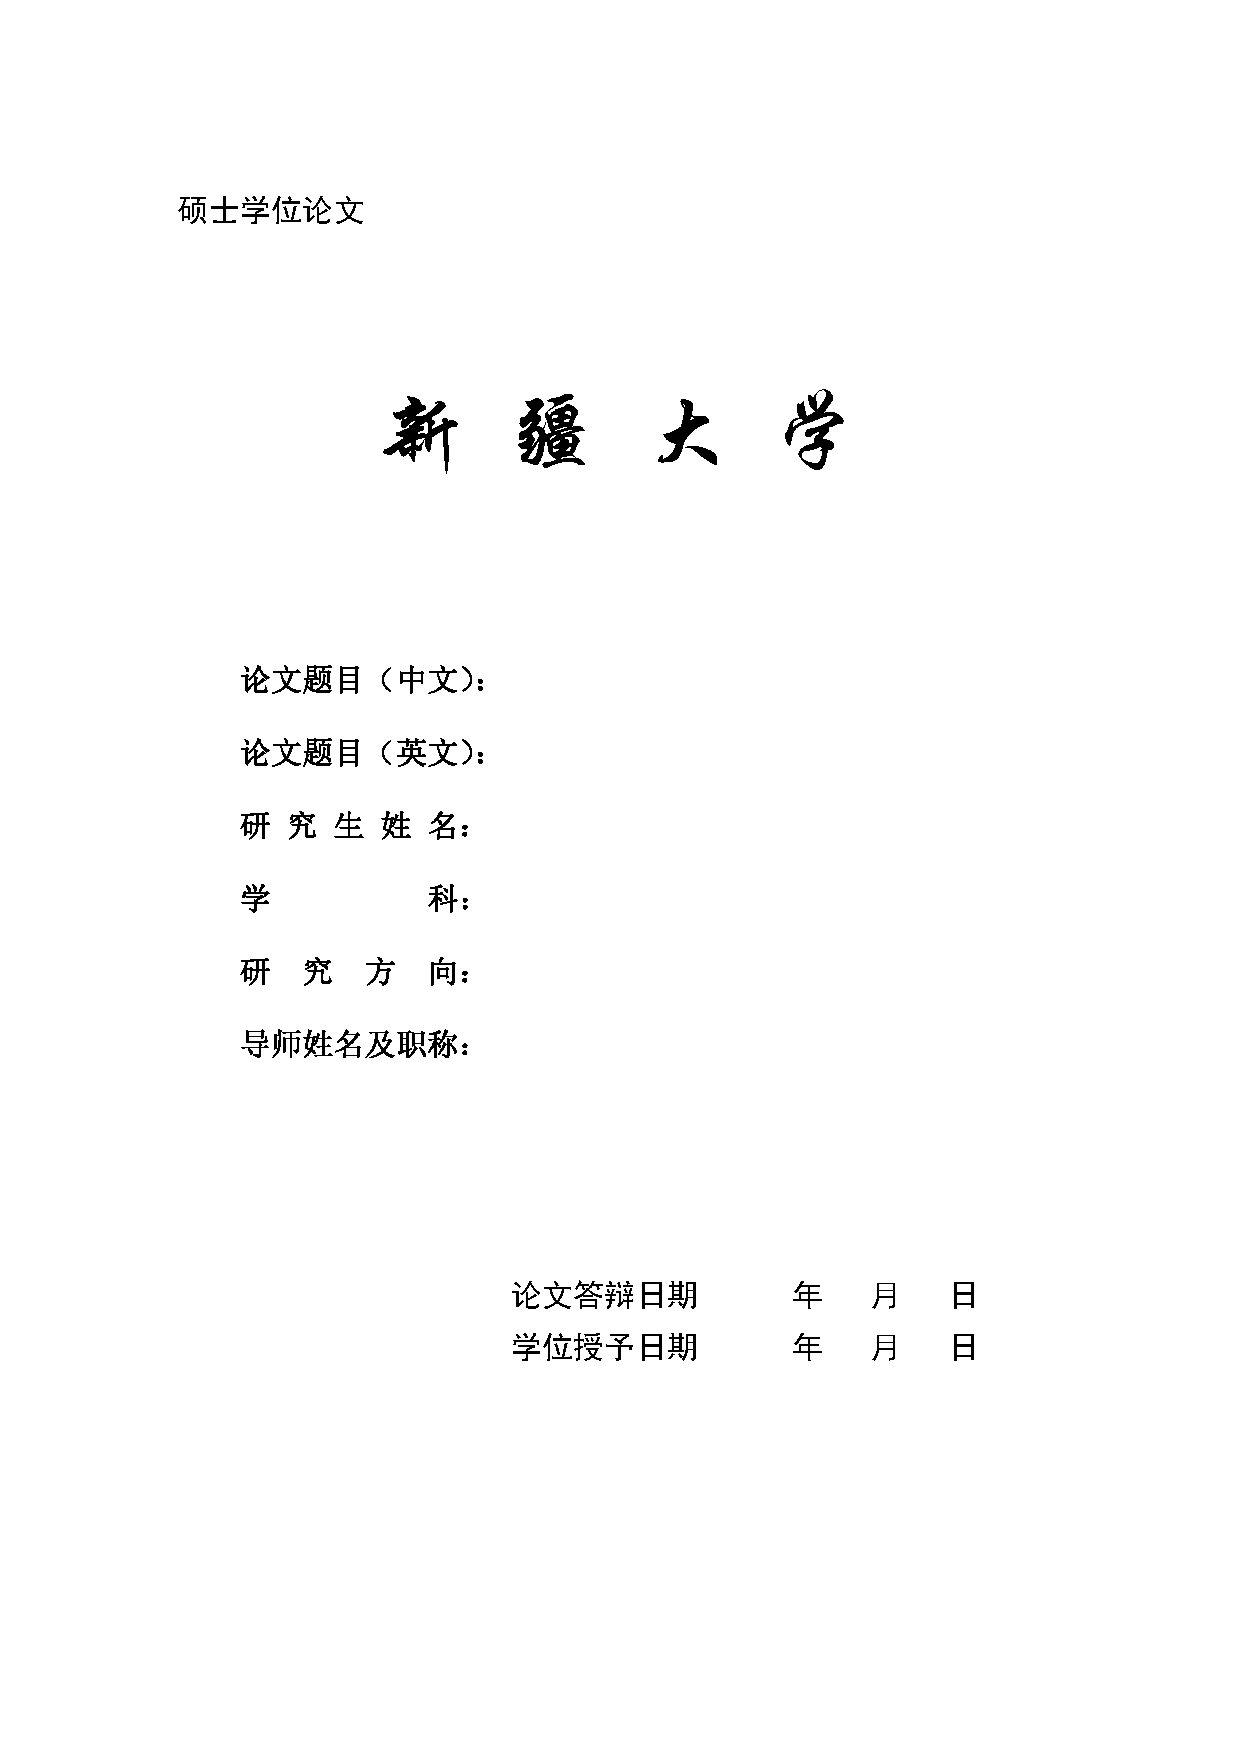
\includepdf{xju_special/xju-master.pdf} % 硕士论文封面   请填写内容后上传pdf

% 使用授权的说明
% \copyrightpage
% 将签字扫描后授权文件 scan-copyright.pdf 替换原始页面
% \copyrightpage[file=scan-copyright.pdf]


\frontmatter
% !TeX root = ../bnuthesis-example.tex

% 中英文摘要和关键字
\setlength{\headheight}{13.70119pt}
\begin{abstract}
食管癌是发生在食管黏膜上皮最常见的恶性肿瘤之一。每年全球约50万例食管癌死亡病例中,中国的食管癌死亡病例占到一半。研究证实,及早发现、准确诊断病灶和对症治疗可有效降低死亡率。内窥镜检查和活检病理切片检查是早期发现及确诊食管癌的“金标准”,然而,随着其成像率的增加,医生阅片负担明显加重,并且医生的诊断存在一定的主观局限性。由于食管癌患者早期的病变症状和外部体征并不明显,对于医疗水平有限的基层医院来说,食管癌的早期诊断,漏诊、误诊率较高。因此,借助计算机进行早期食管癌的自动识别和精准定位对提高诊断率,减少漏诊、误诊率意义重大。计算机辅助诊断一直是计算机科学与医学科学交叉学科研究的热点,实践证明,使用深度学习技术可以为医生提供有效的决策支持,进一步提高诊断的准确性。


  % 关键词用“英文逗号”分隔,输出时会自动处理为正确的分隔符
  \bnusetup{
    keywords = {食管癌诊断; 信息融合; 特征融合; 自注意力机制; 大模型微调}
  }
\end{abstract}

\begin{abstract*}
Esophageal cancer is one of the most common malignant tumors that occurs in the esophageal mucosal epithelium. There are about 500,000 death cases of esophageal cancer worldwide every year, and China accounts for about half of the world's esophageal cancer deaths. Studies have proven that early detection, accurate diagnosis, and treatment of the lesions of esophageal cancer can effectively reduce the mortality rate. Endoscopy and biopsy pathological examination are the “golden standards” for early detection and diagnosis of esophageal cancer. However, with the increase in imaging rates, doctors' burden of reading films has significantly increased, and doctors' diagnosis has a certain degree of subjectivity. Due to the unapparent early lesions and external signs in esophageal cancer patients, early diagnosis of esophageal cancer poses a high risk of missed diagnosis and misdiagnosis in primary hospitals with limited medical capabilities. Therefore, it is of great significance to automatically identify and accurately locate early esophageal cancer by using computers, improving the diagnosis rate and reducing missed diagnoses and misdiagnoses. Computer-aided diagnosis has always been a hot topic in interdisciplinary research between computer science and medical science. The practice has proven that the application of deep learning technology can provide doctors with effective decision-making support and improve diagnostic accuracy.


  % Use comma as separator when inputting
  % 英文关键词首字母请大写
  \bnusetup{
    keywords* = {Esophageal cancer diagnosis; Information fusion; Feature fusion; Self-attention mechanism; Foundation model fine-tuning}
  }
\end{abstract*}


% 目录
\tableofcontents

% 插图和附表清单
% \listoffiguresandtables  % 插图和附表清单
% 如图表较多,可以分别列出清单置于目录页之后。
\listoffigures*           % 插图清单
\listoftables*            % 附表清单

% 符号对照表
% !TeX root = ../thuthesis-example.tex

\begin{denotation}[3cm]

\item[CNNs] 卷积神经网络 (Convolutional Neural Networks)
\item[FCNs] 全卷积网络 (Fully Convolutional Networks)
\item[MLP] 多层感知机 (Multilayer Perceptron)
\item[RNN] 循环神经网络 (Recurrent Neural Network)
\item[NLP] 自然语言处理 (Natural Language Processing)


\end{denotation}



% 也可以使用 nomencl 宏包,需要在导言区
% \usepackage{nomencl}
% \makenomenclature

% 在这里输出符号说明
% \printnomenclature[3cm]

% 在正文中的任意为都可以标题
% \nomenclature{PI}{聚酰亚胺}
% \nomenclature{MPI}{聚酰亚胺模型化合物,N-苯基邻苯酰亚胺}
% \nomenclature{PBI}{聚苯并咪唑}
% \nomenclature{MPBI}{聚苯并咪唑模型化合物,N-苯基苯并咪唑}
% \nomenclature{PY}{聚吡咙}
% \nomenclature{PMDA-BDA}{均苯四酸二酐与联苯四胺合成的聚吡咙薄膜}
% \nomenclature{MPY}{聚吡咙模型化合物}
% \nomenclature{As-PPT}{聚苯基不对称三嗪}
% \nomenclature{MAsPPT}{聚苯基不对称三嗪单模型化合物,3,5,6-三苯基-1,2,4-三嗪}
% \nomenclature{DMAsPPT}{聚苯基不对称三嗪双模型化合物(水解实验模型化合物)}
% \nomenclature{S-PPT}{聚苯基对称三嗪}
% \nomenclature{MSPPT}{聚苯基对称三嗪模型化合物,2,4,6-三苯基-1,3,5-三嗪}
% \nomenclature{PPQ}{聚苯基喹噁啉}
% \nomenclature{MPPQ}{聚苯基喹噁啉模型化合物,3,4-二苯基苯并二嗪}
% \nomenclature{HMPI}{聚酰亚胺模型化合物的质子化产物}
% \nomenclature{HMPY}{聚吡咙模型化合物的质子化产物}
% \nomenclature{HMPBI}{聚苯并咪唑模型化合物的质子化产物}
% \nomenclature{HMAsPPT}{聚苯基不对称三嗪模型化合物的质子化产物}
% \nomenclature{HMSPPT}{聚苯基对称三嗪模型化合物的质子化产物}
% \nomenclature{HMPPQ}{聚苯基喹噁啉模型化合物的质子化产物}
% \nomenclature{PDT}{热分解温度}
% \nomenclature{HPLC}{高效液相色谱(High Performance Liquid Chromatography)}
% \nomenclature{HPCE}{高效毛细管电泳色谱(High Performance Capillary lectrophoresis)}
% \nomenclature{LC-MS}{液相色谱-质谱联用(Liquid chromatography-Mass Spectrum)}
% \nomenclature{TIC}{总离子浓度(Total Ion Content)}
% \nomenclature{\textit{ab initio}}{基于第一原理的量子化学计算方法,常称从头算法}
% \nomenclature{DFT}{密度泛函理论(Density Functional Theory)}
% \nomenclature{$E_a$}{化学反应的活化能(Activation Energy)}
% \nomenclature{ZPE}{零点振动能(Zero Vibration Energy)}
% \nomenclature{PES}{势能面(Potential Energy Surface)}
% \nomenclature{TS}{过渡态(Transition State)}
% \nomenclature{TST}{过渡态理论(Transition State Theory)}
% \nomenclature{$\increment G^\neq$}{活化自由能(Activation Free Energy)}
% \nomenclature{$\kappa$}{传输系数(Transmission Coefficient)}
% \nomenclature{IRC}{内禀反应坐标(Intrinsic Reaction Coordinates)}
% \nomenclature{$\nu_i$}{虚频(Imaginary Frequency)}
% \nomenclature{ONIOM}{分层算法(Our own N-layered Integrated molecular Orbital and molecular Mechanics)}
% \nomenclature{SCF}{自洽场(Self-Consistent Field)}
% \nomenclature{SCRF}{自洽反应场(Self-Consistent Reaction Field)}



% 正文部分
\mainmatter
% !TeX root = ../bnuthesis-example.tex

\chapter{绪论}
\section{研究背景及意义}

\subsection{食管癌及时检出的重要性}
癌症始终是人类生命和健康的严重威胁,近年来癌症的发病率和死亡率均呈持续上升态势,早期发现和精准诊断是提高患者生存率的关键。

食管癌是全球主要的公共卫生问题\cite{liu2017shenmai},被列为全球第八大流行癌症,是癌症相关死亡的第六大原因。 据统计,该疾病每年造成约 572,000 例新病例和 509,000 例死亡\cite{bray2018global},给医疗保健系统带来了沉重负担。 中国的食管癌发病率特别高,其中鳞状细胞癌是主要类型\cite{arnold2015global, wang2018global},在全国所有癌症中发病率排名第三,死亡率排名第四\cite{chen2016national}。食管癌患者的预后很大程度上取决于诊断时癌症的分期和分化程度。 早期食管癌患者手术切除后5年生存率为90\%,比中晚期食管癌患者高出近30\% 。 因此,食管癌的准确诊断对于降低其死亡率至关重要。

食管癌的早期症状不明显,常常被忽视,导致大部分患者在发现时已经进入晚期。目前,食管癌的诊断主要依赖于内窥镜检查和病理学切片检查,这是目前公认的最为准确的诊断手段。早期食管癌是指癌组织生长尚未超过食管壁第二层并且淋巴结中没有癌细胞的阶段,仅局限于食管黏膜和浅表黏膜下层(黏膜下层<500μm的侵袭),未累及肌层,无任何淋巴结转移\cite{ajani2019esophageal}。由于食管癌早期无明显特异性症状,因此对食管癌的诊断主要通过内窥镜检查。内窥镜检查主要是各种内镜的使用,例如常规白光内镜、窄带成像技术(Narrowband Imaging,NBI)和放大内镜、色素内镜、超声内镜(Endoscopic Ultrasound,EUS)等。由于肿瘤标志物\cite{kaz2014epigenetic}检测方式尚缺乏足够的有效的临床经验,内窥镜和病理活检仍是目前诊断早期食管癌的“金标准”。然而,随着医疗技术的进步和检查手段的普及,医生面临的影像数据量急剧增加,使得他们的阅片工作量大大增加,容易出现疏漏和错误。同时,由于医生个体水平和经验的不同,诊断结果存在一定的主观性,且易受到人为因素的影响。因此,为了提高早期食管癌及癌前病变的检出率,借助计算机辅助诊断(Computer Aided Diagnosis,CAD)系统对食管癌进行早期识别和精确定位具有重要意义。临床上食管癌诊断过程如图\ref{诊断}所示。

\begin{figure}
\centering
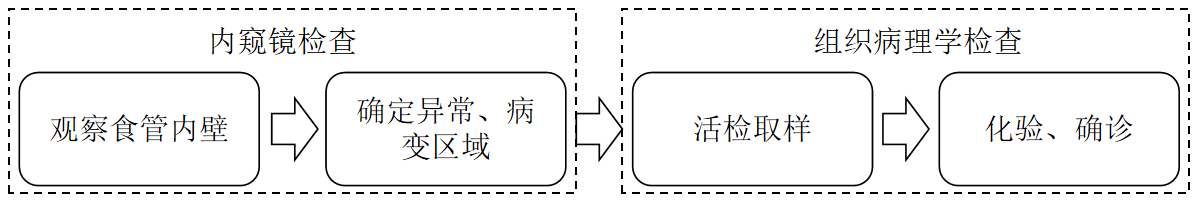
\includegraphics[width=5.5 in]{data/intro_fig/诊断流程001.png}
\caption{食管癌诊断流程图}
\label{诊断}
\end{figure}


\section{引言的写法}

一篇学位论文的引言大致包含如下几个部分:
1、问题的提出;
2、选题背 景及意义;
3、文献综述;
4、研究方法;
5、论文结构安排。
\begin{itemize}
  \item 问题的提出:要清晰地阐述所要研究的问题“是什么”。
    \footnote{选题时切记要有“问题意识”,不要选不是问题的问题来研究。}
  \item 选题背景及意义:论述清楚为什么选择这个题目来研究,即阐述该研究对学科发展的贡献、对国计民生的理论与现实意义等。
  \item 文献综述:对本研究主题范围内的文献进行详尽的综合述评,“述”的同时一定要有“评”,指出现有研究状态,仍存在哪些尚待解决的问题,讲出自己的研究有哪些探索性内容。
  \item 研究方法:讲清论文所使用的学术研究方法。
  \item 论文结构安排:介绍本论文的写作结构安排。
\end{itemize}


% !TeX root = ../bnuthesis-example.tex

\chapter{全局-局部层次融合的食管癌分期分类}
% \setcounter{figure}{20} % 重新设置图号计数器

 
% !TeX root = ../bnuthesis-example.tex

\chapter{内镜-病理信息融合的食管癌分化程度分类}
% \setcounter{figure}{27} % 重新设置图号计数器
% \setcounter{table}{9} % 重新设置表格计数器

% !TeX root = ../bnuthesis-example.tex

\chapter{中心-周边多粒度融合的食管癌内镜图像分割}
% \setcounter{figure}{32} % 重新设置图号计数器
% \setcounter{table}{13} % 重新设置表格计数器

\chapter{领域知识微调融合的食管病灶分割}
% \setcounter{figure}{40} % 重新设置图号计数器
% \setcounter{table}{21} % 重新设置表格计数器

\chapter{总结与展望}
% \setcounter{figure}{44} % 重新设置图号计数器



% 其他部分
\backmatter

% 参考文献
\bibliography{ref/refs}  % 参考文献使用 BibTeX 编译
% \printbibliography       % 参考文献使用 BibLaTeX 编译

% 附录
% 本科生需要将附录放到声明之后,个人简历之前
%\appendix
%% !TeX root = ../bnuthesis-example.tex

\chapter{补充内容}

附录是与论文内容密切相关、但编入正文又影响整篇论文编排的条理和逻辑性的资料,例如某些重要的数据表格、计算程序、统计表等,是论文主体的补充内容,可根据需要设置。

附录中的图、表、数学表达式、参考文献等另行编序号,与正文分开,一律用阿拉伯数字编码,
但在数码前冠以附录的序号,例如“图~\ref{fig:appendix-figure}”,
“表~\ref{tab:appendix-table}”,“式\eqref{eq:appendix-equation}”等。


\section{插图}

% 附录中的插图示例(图~\ref{fig:appendix-figure})。

\begin{figure}
  \centering
  
\includegraphics[width=0.6\linewidth]{example-image-a.pdf}
  \caption{附录中的图片示例}
  \label{fig:appendix-figure}
\end{figure}


\section{表格}

% 附录中的表格示例(表~\ref{tab:appendix-table})。

\begin{table}
  \centering
  \caption{附录中的表格示例}
  \begin{tabular}{ll}
    \toprule
    文件名          & 描述                         \\
    \midrule
    bnuthesis.dtx   & 模板的源文件,包括文档和注释 \\
    bnuthesis.cls   & 模板文件                     \\
    bnuthesis-*.bst & BibTeX 参考文献表样式文件    \\
    bnuthesis-*.bbx & BibLaTeX 参考文献表样式文件  \\
    bnuthesis-*.cbx & BibLaTeX 引用样式文件        \\
    \bottomrule
  \end{tabular}
  \label{tab:appendix-table}
\end{table}


\section{数学表达式}

% 附录中的数学表达式示例(式\eqref{eq:appendix-equation})。
\begin{equation}
  \frac{1}{2 \uppi \symup{i}} \int_\gamma f = \sum_{k=1}^m n(\gamma; a_k) \mathscr{R}(f; a_k)
  \label{eq:appendix-equation}
\end{equation}


\section{文献引用}

附录\cite{dupont1974bone}中的参考文献引用\cite{zhengkaiqing1987}示例
\cite{dupont1974bone,zhengkaiqing1987}。

\printbibliography



% 个人简历、在学期间完成的相关学术成果
% 本科生可以附个人简历,也可以不附个人简历
% !TeX root = ../bnuthesis-example.tex

\begin{resume}

  \section*{个人简历}

霍相佐,男,汉族;2021年就读于新疆大学计算机科学与技术学院,计算机科学与技术专业,研究方向为医学图像处理。


  \section*{在学期间的第一作者学术论文}

  \begin{achievements}
    \item Huo X, Tian S, Yang Y, et al. SPA: Self-Peripheral-Attention for central–peripheral interactions in endoscopic image classification and segmentation[J]. \textbf{Expert Systems with Applications}, 2024, 245: 123053.(中科院一区Top,SCI源刊,IF:8.5)--(第五章引用)
    \item Huo X, Sun G, Tian S, et al. HiFuse: Hierarchical multi-scale feature fusion network for medical image classification[J]. \textbf{Biomedical Signal Processing and Control}, 2024, 87: 105534.(中科院二区,SCI源刊,IF:5.1)--(第三章引用)

  \end{achievements}


  \section*{科研项目}
    
基于特征融合的多源食管癌诊断算法研究(主持), 优秀博士生科研创新项目(XJU2022BS078);

多模态食管癌知识图谱构建和自动识别关键技术研究(参与), 国家自然科学基金(62162058)。


\end{resume}


% 致谢
% !TeX root = ../bnuthesis-example.tex

\begin{acknowledgements}
祝大家:身体健康!事业有成!阖家幸福!龙年吉祥!
\end{acknowledgements}


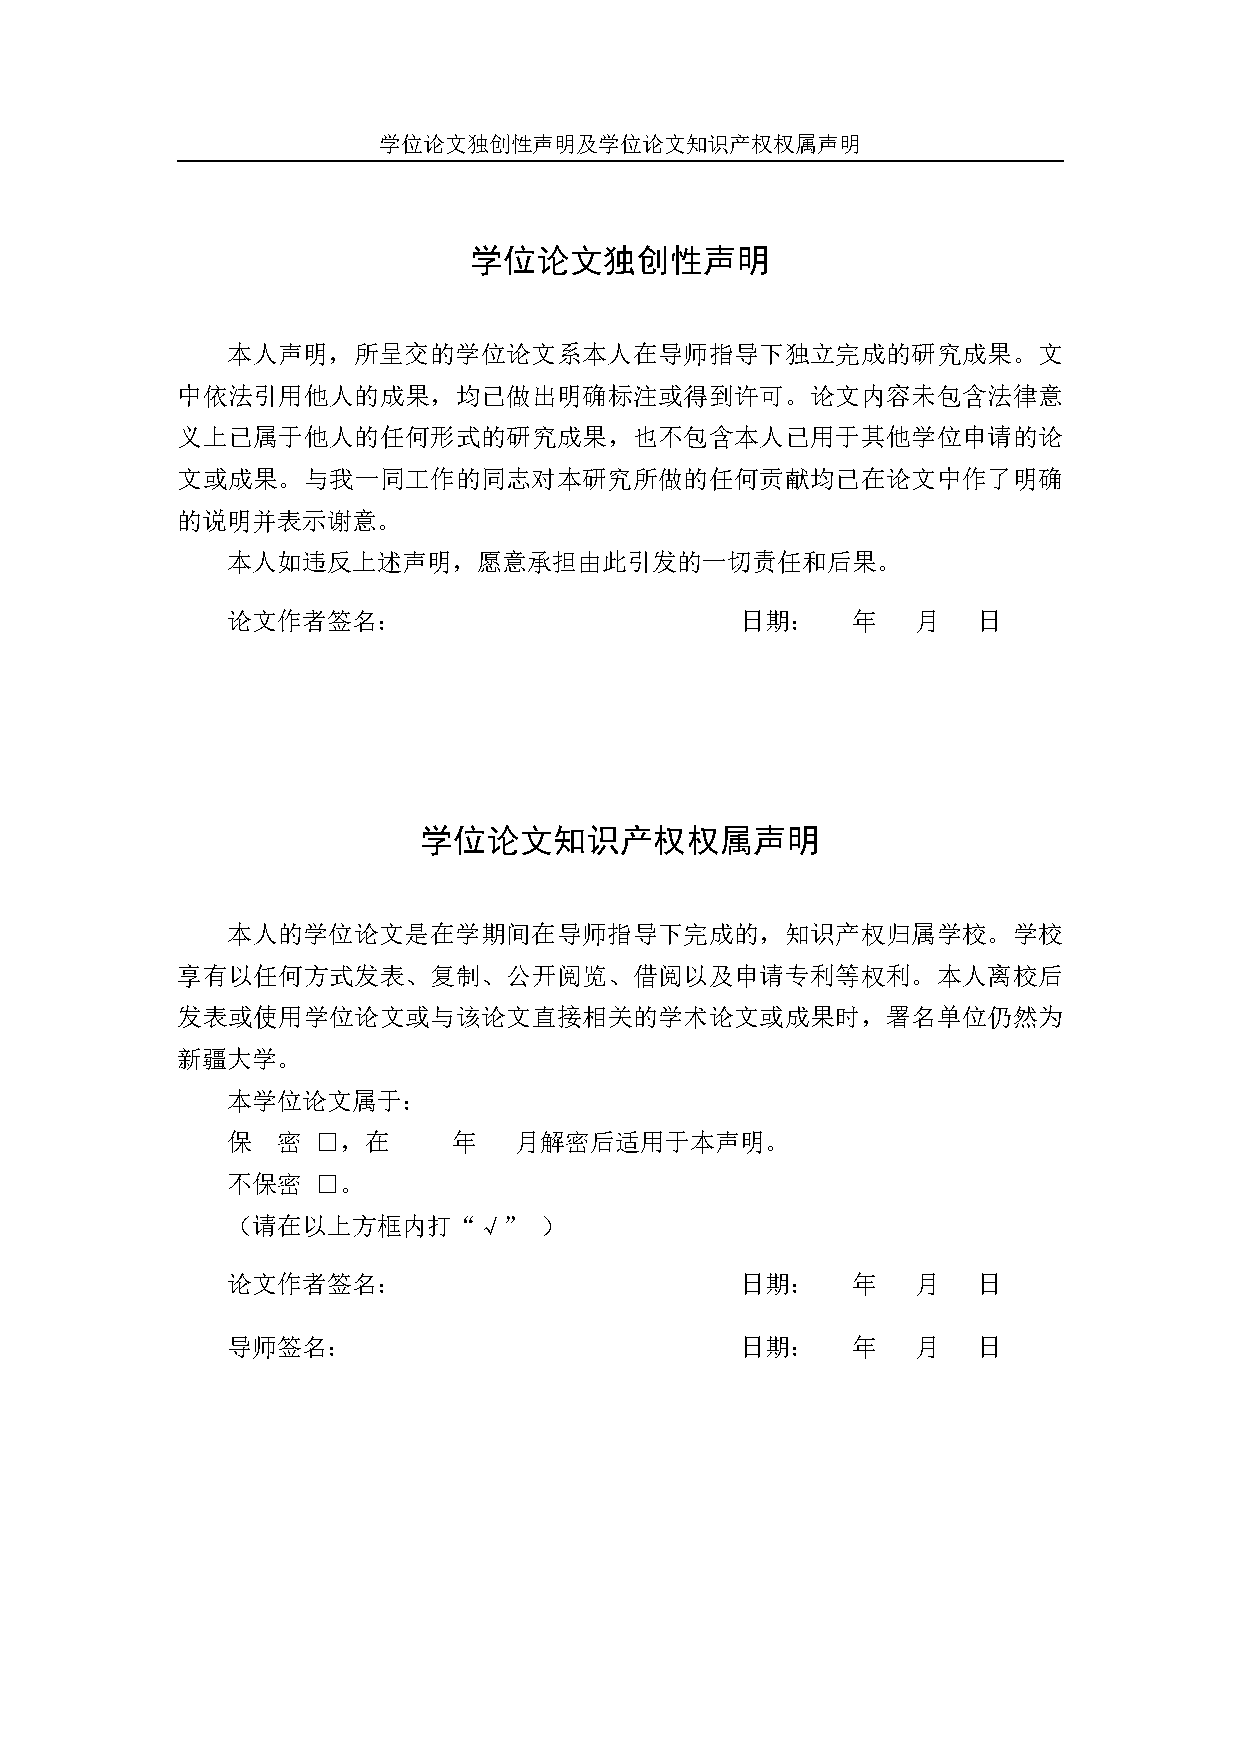
\includepdf{xju_special/xju-declaration.pdf} % 请填写内容后上传pdf

\end{document}
